% Copyright 2021 Politecnico di Milano, Italy. Inc. All rights reserved.

\documentclass[11pt,a4paper,twocolumn]{article}

% === Packages and configurations ===
% Titles
\usepackage{titlesec}
\usepackage{color}
\usepackage{fix-cm}

% Language and fonts
\usepackage[utf8]{inputenc}
\usepackage[english]{babel}
\usepackage[T1]{fontenc} % Font encoding

% Images
\usepackage{graphicx}
\graphicspath{{Images/}} % Path for images' folder
\usepackage{eso-pic} % For the background picture on the title page
\usepackage{subfig} % Numbered and caption subfigures using \subfloat
\usepackage[font=scriptsize]{caption} % Coloured captions
\usepackage{transparent}

% Math
\usepackage{amsmath}
\usepackage{amsthm}
\usepackage{bm}
\usepackage[overload]{empheq}  % For braced-style systems of equations

% Tables
\usepackage{tabularx}

\usepackage{longtable} % tables that can span several pages
\usepackage{colortbl}

% Algorithms
\usepackage{algorithm}
\usepackage{algorithmic}

% Bibliography and references
\usepackage[colorlinks=true,linkcolor=black,anchorcolor=black,citecolor=black,filecolor=black,menucolor=black,runcolor=black,urlcolor=black]{hyperref} % Adds clickable links at references
\usepackage{cleveref}
\usepackage[square, numbers, sort&compress]{natbib} % Square brackets, citing references with numbers, citations sorted by appearance in the text and compressed
\bibliographystyle{plain} % You may use a different style adapted to your field

% Appendix
\usepackage{appendix}

% Bullet lists
\usepackage{enumitem}

% Other
\usepackage{amsthm,thmtools,xcolor} % Coloured "Theorem"
\usepackage{comment} % Comment part of code
\usepackage{fancyhdr} % Fancy headers and footers
\usepackage{lipsum} % Insert dummy text
\usepackage{tcolorbox} % Create colored boxes (e.g. the one for the keywords)
\usepackage{stfloats} % Correct position of the tables

% === New commands ===
\newcommand{\bea}{\begin{eqnarray}} % Shortcut for equation arrays
\newcommand{\eea}{\end{eqnarray}}
\newcommand{\e}[1]{\times 10^{#1}}  % Powers of 10 notation
\newcommand{\mathbbm}[1]{\text{\usefont{U}{bbm}{m}{n}#1}} % From mathbbm.sty
\newcommand{\pdev}[2]{\frac{\partial#1}{\partial#2}}

% === Title settings ===
% Set the geometric layout of the document
\usepackage{geometry}
\geometry{
  top=3cm,
  left = 1.5cm,
  right = 1.5cm,
  bottom=2cm,
  headheight= 2cm,
  headsep= 0cm,
}
\raggedbottom 

% Create color bluePoli (-> manuale grafica coordinata:  https://www.polimi.it/fileadmin/user_upload/il_Politecnico/grafica-coordinata/2015_05_11_46xy_manuale_grafica_coordinata.pdf)
\definecolor{bluePoli}{cmyk}{0.4,0.1,0,0.4}

% Custom theorem environments
\declaretheoremstyle[
  headfont=\color{bluePoli}\normalfont\bfseries,
  bodyfont=\color{black}\normalfont\itshape,
]{colored}

\captionsetup[figure]{labelfont={color=bluePoli}} % Set colour of the captions
\captionsetup[table]{labelfont={color=bluePoli}} % Set colour of the captions
\captionsetup[algorithm]{labelfont={color=bluePoli}} % Set colour of the captions

\theoremstyle{colored}
\newtheorem{theorem}{Theorem}[section]
\newtheorem{proposition}{Proposition}[section]

% Enhances the features of the standard "table" and "tabular" environments.
\newcommand\T{\rule{0pt}{2.6ex}}
\newcommand\B{\rule[-1.2ex]{0pt}{0pt}}

% Algorithm description
\newcounter{algsubstate}
\renewcommand{\thealgsubstate}{\alph{algsubstate}}
\newenvironment{algsubstates}{
    \setcounter{algsubstate}{0}%
    \renewcommand{\STATE}{%
    \stepcounter{algsubstate}%
    \Statex {\small\thealgsubstate:}\space}
    }{}
    
% Custom theorem environment
\newcolumntype{L}[1]{>{\raggedright\let\newline\\\arraybackslash\hspace{0pt}}m{#1}}
\newcolumntype{C}[1]{>{\centering\let\newline\\\arraybackslash\hspace{0pt}}m{#1}}
\newcolumntype{R}[1]{>{\raggedleft\let\newline\\\arraybackslash\hspace{0pt}}m{#1}}

% Custom itemize environment
\setlist[itemize,1]{label=$\bullet$}
\setlist[itemize,2]{label=$\circ$}
\setlist[itemize,3]{label=$-$}
\setlist{nosep}

% Set separation of columns 
\setlength{\columnsep}{30pt}

% Create command for background pic
\newcommand\BackgroundPic{% Adding background picture
	\put(198,330){
		\parbox[b][\paperheight]{\paperwidth}{%
			\vfill
			\centering
			\transparent{0.4}
			
\includegraphics[width=0.7\paperwidth]{raggiera_polimi.eps}%
			\vfill
}}}

% Set indentation
\setlength\parindent{0pt}

% Custom title commands
\titleformat{\section}
{\color{bluePoli}\normalfont\Large\bfseries}
{\color{bluePoli}\thesection.}{1em}{}
\titlespacing*{\section}
{0pt}{2ex}{1ex}

\titleformat{\subsection}
{\color{bluePoli}\normalfont\large\bfseries}
{\color{bluePoli}\thesubsection.}{1em}{}
\titlespacing*{\subsection}
{0pt}{2ex}{1ex}

% Custom headers and footers
\pagestyle{fancy}
\fancyhf{}
      
\fancyfoot{}
\fancyfoot[C]{\thepage} % page
\renewcommand{\headrulewidth}{0mm} % headrule width
\renewcommand{\footrulewidth}{0mm} % footrule width

\makeatletter
\patchcmd{\headrule}{\hrule}{\color{black}\hrule}{}{} % headrule
\patchcmd{\footrule}{\hrule}{\color{black}\hrule}{}{} % footrule
\makeatother

% -> Create the header
\chead[C]{
\centering
\begin{tcolorbox}[arc=0pt, boxrule=0pt, colback=bluePoli!60, width=\textwidth, colupper=white]
    \textsc{\textbf{Executive summary}} \hfill \textsc{\textbf{\author}} 
\end{tcolorbox}
}

\renewcommand{\title}{Ray Distribution Aware Heuristics for Bounding Volume Hierarchies Construction in Ray Tracing}
\renewcommand{\author}{Lapo Falcone}
\newcommand{\course}{Computer Science and Engineering - Ingegneria Informatica}
\newcommand{\advisor}{Prof. Marco Gribaudo}
\newcommand{\YEAR}{2023-24}

% === Start of document ===
\begin{document}

% Title page
% DO NOT REMOVE SPACES BETWEEN LINES!

\twocolumn[{\begin{@twocolumnfalse}

\AddToShipoutPicture*{\BackgroundPic}

\vspace{-1.5cm}
\hspace{-0.6cm}
\includegraphics[width=0.6\textwidth]{logo_polimi_ing_indinf.eps}

\vspace{-1mm}
\fontsize{0.3cm}{0.5cm}\selectfont \bfseries \textsc{\color{bluePoli} Executive Summary of the Thesis}\\

\vspace{-0.2cm}
\Large{\textbf{\color{bluePoli}{\title}}}\\

\vspace{-0.2cm}
\fontsize{0.3cm}{0.5cm}\selectfont \bfseries \textsc{\color{bluePoli} Laurea Magistrale in \course}\\

\vspace{-0.2cm}
\fontsize{0.3cm}{0.5cm} \normalfont Author: \textsc{\textbf{\author}} \hspace{1cm}
\fontsize{0.3cm}{0.5cm} \normalfont Advisor: \textsc{\textbf{\advisor}} \hspace{1cm}
\fontsize{0.3cm}{0.5cm} \normalfont Academic year: \textsc{\textbf{\YEAR}}

\small \normalfont

\vspace{11pt}

\centerline{\rule{1.0\textwidth}{0.4pt}}

\vspace{15pt}
\end{@twocolumnfalse}}]

\thispagestyle{plain} % In order to not show the header in the first page

\pagebreak
\fontsize{10.1pt}{0.45cm}\selectfont
\section{Introduction}
Our thesis is set in the context of computer graphics, in particular ray tracing. With this work, we aim to improve the performance of a core structure present in any ray tracing algorithm, namely the Bounding Volume Hierarchy (BVH), a binary tree whose nodes usually are Axis-Aligned Bounding Boxes (AABB). A BVH is used to find the intersections between a ray and the scene, which is a fundamental step in the process of tracing the path of a ray from a light source to the camera.

In the state of the art, BVHs are built with a greedy algorithm based on two heuristics: Surface Area Heuristic (SAH) \cite{sah}, and Longest Splitting Plane Heuristic (LSPH). These two heuristics aim to locally minimize the cost of traversing a level of the BVH, and are based on some hypotheses, the most important of which is that the ray distribution in the scene is uniform.

BVHs aren't the only optimization used in ray tracing. Indeed a Monte-Carlo variance reduction technique is used to reduce the number of rays needed to achieve a high-quality rendering. This technique is called Importance Sampling \cite{importance_sampling}, and a specialization of it, namely Next Event Estimation (NEE), generates artifacts in the ray distribution in the scene.

This means that the SAH hypothesis falls: our work tries to leverage the knowledge of the non-uniform ray distribution, in order to build better BVHs than those that could be built by using SAH and LSPH. We propose two novel heuristics, namely Projected Area Heuristic (PAH) and Splitting Plane Facing Heuristic (SPFH), and a top level structure to enable their use, along with an in-depth analysis of the experimental results of the tests we performed by using a framework developed by us in modern C++.

In this executive summary, we briefly touch on the main points of our work, starting from the background theory needed to understand it, passing through the proposed novelties and their implementation, and getting to an overview of the experimental results.

\section{Background Theory}
Ray tracing is a family of techniques that, starting from a mathematical representation of a scene, is capable of performing an approximated light transport simulation to render an image. In order to simulate light transport, the main algorithm of any ray tracer consists of the following steps:
\begin{enumerate}
    \item Cast rays from the light sources present in the scene;
    \item For each ray, find the first collision with an object of the scene;
    \item Based on the material of the object, decrease the energy of the ray, and make it bounce to a different direction;
    \item This process is recursively carried out until the ray loses all its energy, or it hits the camera;
    \item If the ray hits the camera, color the hit pixel based on the energy the ray is carrying.
\end{enumerate}

\begin{figure}[H]
    \centering
    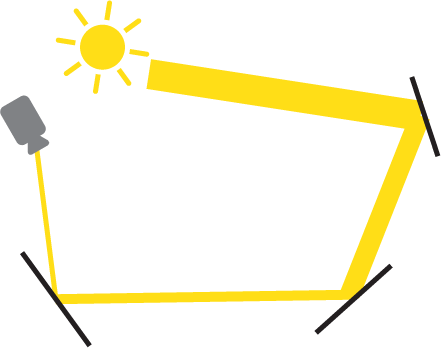
\includegraphics[width=\textwidth*\real{0.22}]{Images/ray_tracing_simple.png}
    \caption{2D ray tracing visualization.}
    \label{fig:ray_tracing_simple}
\end{figure}

Many of the rays cast from light sources end up not hitting the camera, therefore they are wasted. For this reason, in many ray tracing techniques the process is carried out in the opposite direction: the light rays are cast from the camera, and bounce around the scene until they hit a light source. These techniques fall under the name of backward ray tracing, and work thanks to the light reciprocity principle, which states that light transmits in the same way in both directions. From now on, when we refer to ray tracing, we implicitly reference backward ray tracing.

While ray tracing, at its core, is very simple, a lot of research effort has been put into making it faster. The main problem with light simulation is that, in the real world, a huge amount of rays\footnote{A $100W$ lightbulb produces around $10^{20}$ photons per second.} is cast, in the form of photons, and are then captured by our eyes or a digital camera to produce an image. For this reason, one important family of optimizations has as its main goal to reduce the number of rays needed to produce an accurate image.

\subsection{Kajiya and Monte-Carlo}
In order to understand better how these optimizations work, we first have to understand the Kajiya's rendering equation \cite{rendering_equation}, which concisely describes how light transport works:

\begin{subequations}
    \begin{align*}
        L_o(\bar{x},&\bar{\omega}_o) = L_e(\bar{x}, \bar{\omega}_o) +\\
        &+\int_\Omega b(\bar{x}, \bar{\omega}_i, \bar{\omega}_o) \cdot \cos(\bar{n}, \bar{\omega}_i) \cdot L_i(\bar{x}, \bar{\omega}_i) d\bar{\omega}_i
    \end{align*}
\end{subequations}

In synthesis, this equation tells us that the amount of light exiting a point $\bar{x}$ toward direction $\bar{\omega}_o$ is given by a constant emission term $L_e$, summed to a reflective term, described by an integral over a hemisphere $\Omega$,

The integral term computes how much light the point $\bar{x}$ is receiving from all the directions of the hemisphere oriented toward the normal $\bar{n}$ to the surface the point is part of. Then, it uses the BRDF function $b$ to calculate how much of the light entering the point is reflected toward the direction $\bar{\omega}_o$.

The integral term is recursive, indeed, the light entering the point from a given direction $\bar{\omega}_i$, corresponds to the light exiting another point.

\begin{figure}[H]
    \centering 
    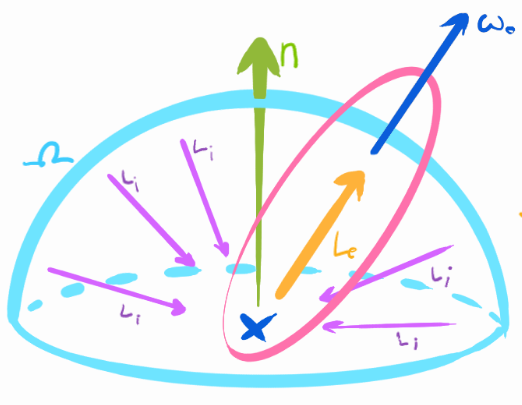
\includegraphics[width=\textwidth*\real{0.225}]{Images/kajiya_visual.png}
    \caption{Kajiya's equation terms.}
    \label{fig:kajiya_recursiveness}
\end{figure}

The task of any ray tracer is to numerically approximate the Kajiya's equation for any point of the scene, in order to, eventually, find out how much light each point reflects toward the direction of the focal point of the camera.

Computing the emissive term $L_e$, knowing where the light sources are located, is trivial; the most time-consuming part is to resolve the integral. In order to do so, Monte-Carlo integration is used. In this summary we assume that Monte-Carlo integration is known by the reader, and we focus mostly on how to apply it to the ray tracing context. In particular, to estimate the light entering the point hit by a view ray\footnote{An initial ray originating at the camera.}, we can cast a certain amount of probe rays toward random directions. The probe rays will hit other points, where other probe rays will be cast, recursively, until the probe rays lose all their energy\footnote{In practice, after a certain recursion threshold.}, or they hit a light source.

The more probe rays we cast, the more the estimation of the light entering a point is accurate, and, consequently, the rendered image. The issue is that, by a fundamental Monte-Carlo estimator property, to cut the estimation error in half, we need 4 times more probe rays. For this reason, some variance reduction techniques have been developed to reduce error without increasing the number of rays.

The variance reduction technique relevant for this thesis is called \textit{importance sampling}. Instead of casting the probe rays toward uniformly random directions, we cast them by following a non-uniform Probability Density Function (PDF). The PDF should be proportional to the integrand function but, since it is unknown, we can approximate it by casting more rays directly toward light sources. This importance sampling method is called \textit{light sampling}, or \textit{Next Event Estimation} (NEE).

NEE makes it so that the ray distribution inside the scene is not uniform, but it is more dense in proximity to light sources. This is a core hypothesis of our work.

\subsection{BVHs}
Until now, we have assumed we know where a ray intersects an object of the scene. In the real world, this is not the case, and finding the ray-scene intersection is a task common to any ray tracing algorithm. For this reason, the second big family of optimizations is to find a way to accelerate this process. In the vast majority of graphics applications, the scene is described by a huge amount of triangles, approximating the surfaces of the objects. An object formed by triangles is called a mesh.

Therefore, the problem of finding the ray-scene intersection can be reduced to the problem of ray-triangle intersection, which has a known and very optimized solution. The first, naive, way of finding the intersection between a ray and the scene is a brute-force loop over all the triangles present in the scene. However, the complexity of this method increases linearly with the number of triangles or the number of rays in the scene. 

A better technique, which is used in state-of-the-art ray tracers, is to organize the triangles hierarchically, in a spatial binary tree called Bounding Volume Hierarchy (BVH). The idea is to divide the scene into two parts, and enclose the triangles inside each one into two parallelepipeds aligned with the cartesian axes, called Axis-Aligned Bounding Boxes (AABB). Now, if a ray doesn't intersect an AABB, it won't intersect any of the triangles inside it, therefore AABBs can be used as rejection tests. In a BVH, this simple idea is applied recursively: the scene is divided into two AABBs, then each one is further divided into two, and so on, until a stopping criterion is met. 

With a balanced BVH, finding the ray-scene intersection becomes logarithmic with reference to the number of triangles, and is therefore a big improvement over the brute-force approach, considering how many rays are cast.

Building the BVH optimally is an NP-complete problem, therefore, in real-world applications, a greedy algorithm and heuristics are used to make the problem tractable. In particular, the heuristics are used to decide along which axis to cut the AABB, and to decide how to split the triangles into the two children nodes.

The first heuristic used in state-of-the-art applications is the Longest Splitting Plane Heuristic (LSPH), where the AABB is cut with a plane perpendicular to its longest dimension. It is worth noting that, in all the state-of-the-art builders, only the three cartesian plane orientations are taken into consideration. In other words, it is not possible to cut the AABB with an oblique plane, as it wouldn't make sense when the AABBs are, indeed, axis-aligned.

The second heuristic is Surface Area Heuristic (SAH). With SAH, when the builder has to split the triangles by using the plane orientation selected by LSPH, it tries many different options\footnote{Binned approach.}, and assigns to each one a cost, which can be computed via this formula:

$$
Cost(Aabb) = \frac{SurfaceArea_{Aabb}}{SurfaceArea_{root}} \cdot \#triangles_{Aabb} \cdot K
$$

In summary, the formula tries to approximate the probability that the AABB is hit by a random ray, and weights it with the number of triangles in the node and a constant. The split with the lowest combined cost (i.e. hit probability) among the two AABBs gets greedily chosen.

The fact that the hit probability can be computed as $\frac{SurfaceArea_{Aabb}}{SurfaceArea_{root}}$ has as hypothesis that the rays are uniformly randomly distributed in the scene. However, as we noted while talking about importance sampling, we know this is not the case.

\section{Projected Area Heuristic}
The first novelty we propose in our work is the Projected Area Heuristic (PAH). The core principle behind PAH is to try to estimate better the hit probability of an AABB, by leveraging the knowledge about the ray distribution in the scene, caused by light importance sampling. In particular, we take into account two possible ray distributions:
\begin{description}
    \item[Parallel ray distributions] arise in proximity of planar area light sources;
    \item[Radial ray distributions] arise in proximity of point light sources, such as spotlights. 
\end{description}

\begin{figure}[H]
    \centering
    \subfloat[Parallel]{
        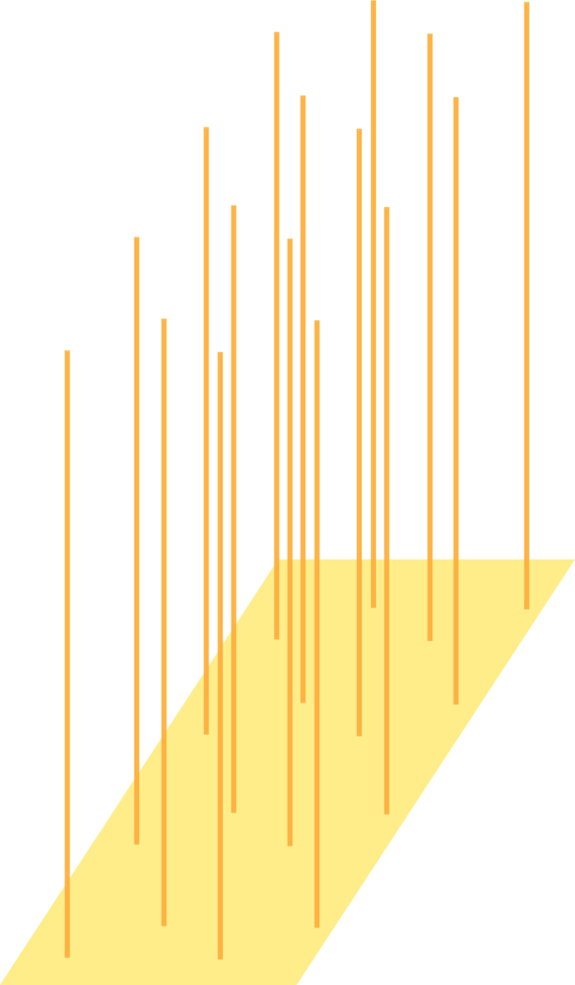
\includegraphics[width=\textwidth*\real{0.1}]{Images/plane_light_rays.png}
	}
	\qquad
	\subfloat[Radial]{
        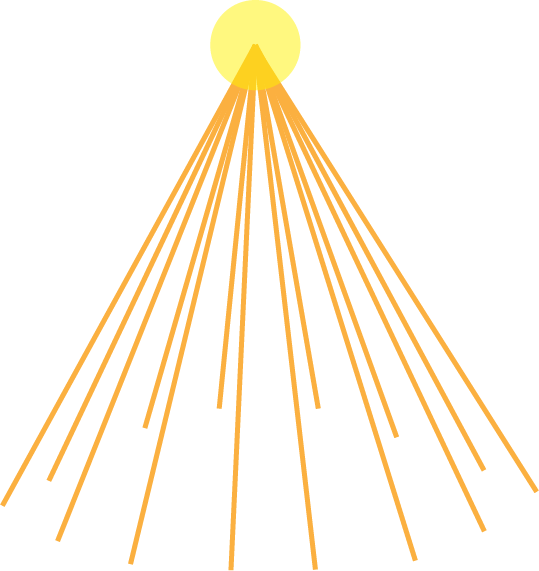
\includegraphics[width=\textwidth*\real{0.15}]{Images/point_light_rays.png} 
    }
    \caption{Ray distributions.}
    \label{fig:ray_distributions}
\end{figure} 

If one of these ray distributions is present in a given region of the scene, then we can better estimate the probability a ray hits an AABB present in this region by projecting the AABB: in the case of parallel rays, the projection is orthographic, whereas, for radial rays, the projection is perspective.

\begin{figure}[H]
    \centering 
    \subfloat[Orthographic]{
        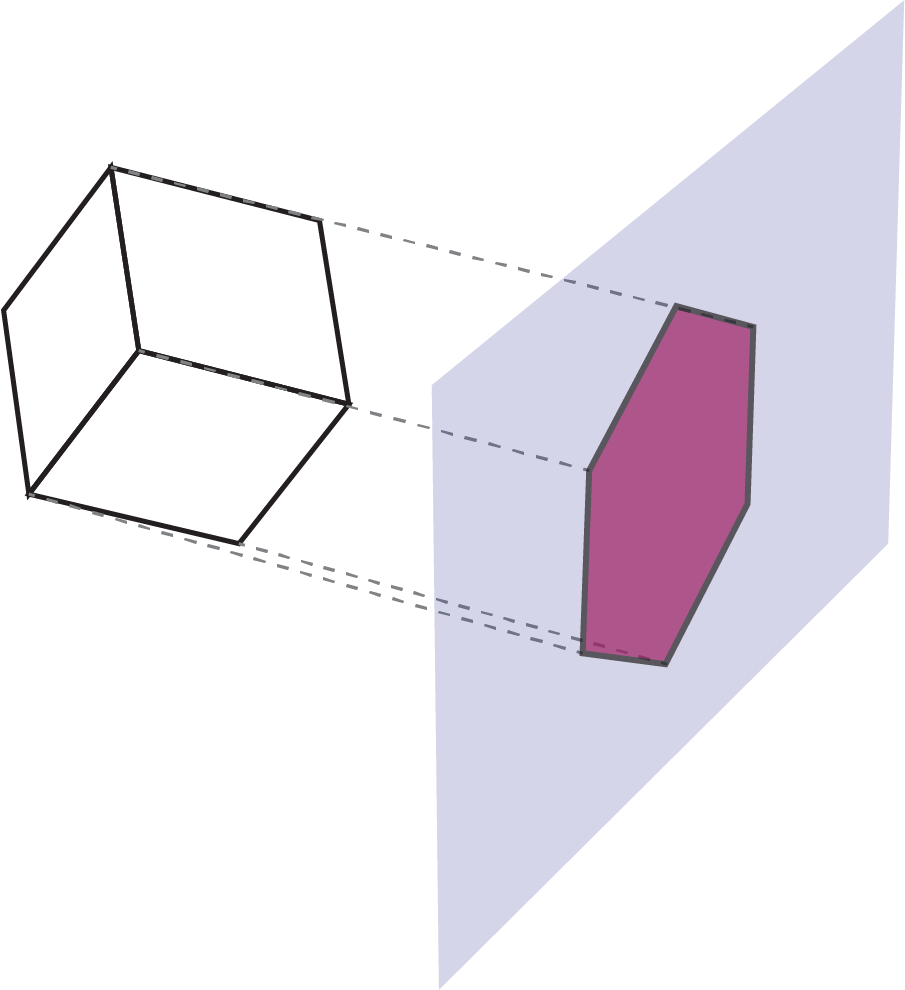
\includegraphics[width=\textwidth*\real{0.12}]{Images/ortho_projection.png}
	}
	\qquad
	\subfloat[Perspective]{
        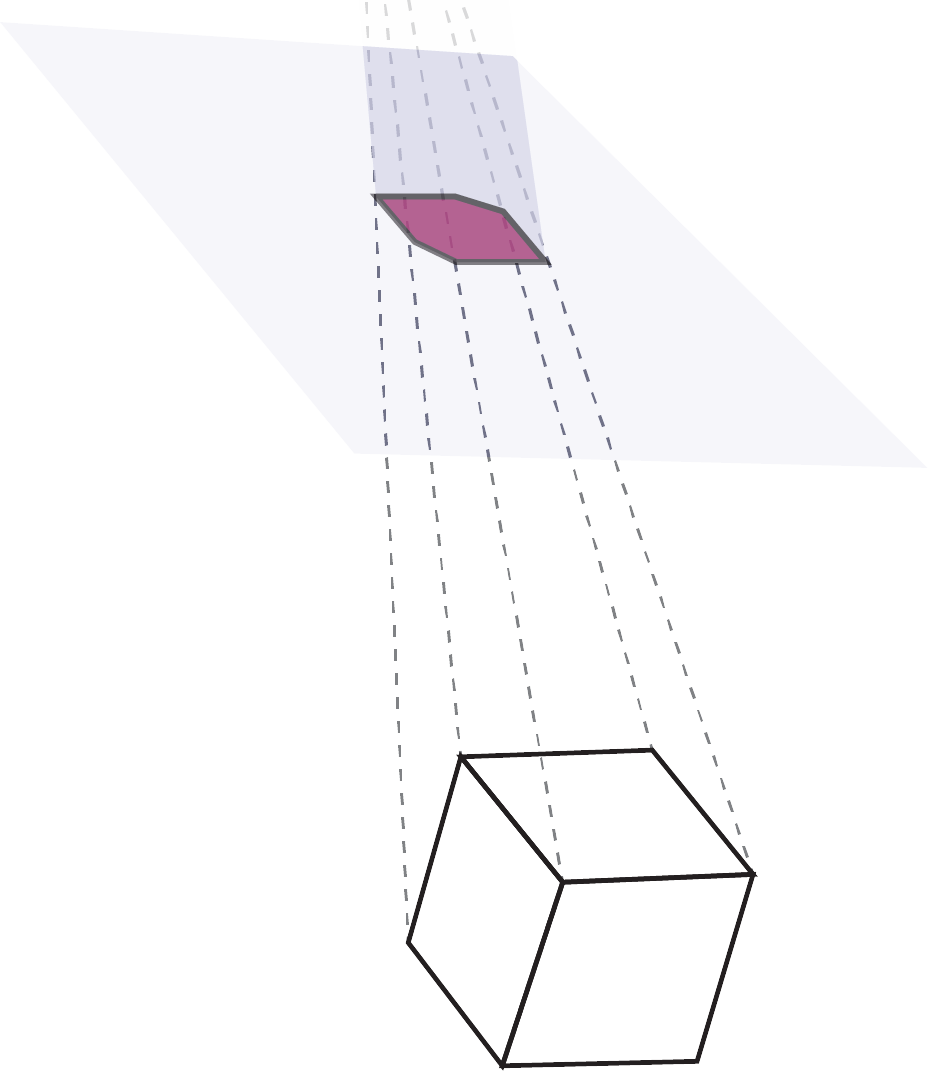
\includegraphics[width=\textwidth*\real{0.17}]{Images/perspective_projection.png} %TODO improve image
    }
    \caption{Projections.}
    \label{fig:projections}
\end{figure}

\section*{4. Splitting Plane Facing Heuristic}
The second novel heuristic we propose is a possible alternative to LSPH, and is called Splitting Plane Facing Heuristic (SPFH). It is based on the same considerations we made for PAH, but it is applicable to how to decide the orientation of the splitting plane, and takes into consideration if the AABB is in a region with a parallel or radial ray distribution.

As described by \cite{bvh_overlapping_metric}, a large 3D overlap between children nodes, leads to a low-quality BVH. With SPFH, we try to minimize the overlap between children nodes in the 2D space of their projections. The idea is based on the observation that, if the splitting plane is perpendicular to a ray, there is a large probability that the ray will intersect both the resulting children AABBs. Conversely, if the plane is parallel to a ray, it is not probable that it will hit both, because the overlap of their projections will be a lot smaller in many scenarios.

\begin{figure}[H]
    \centering 
    \subfloat[Perpendicular]{
        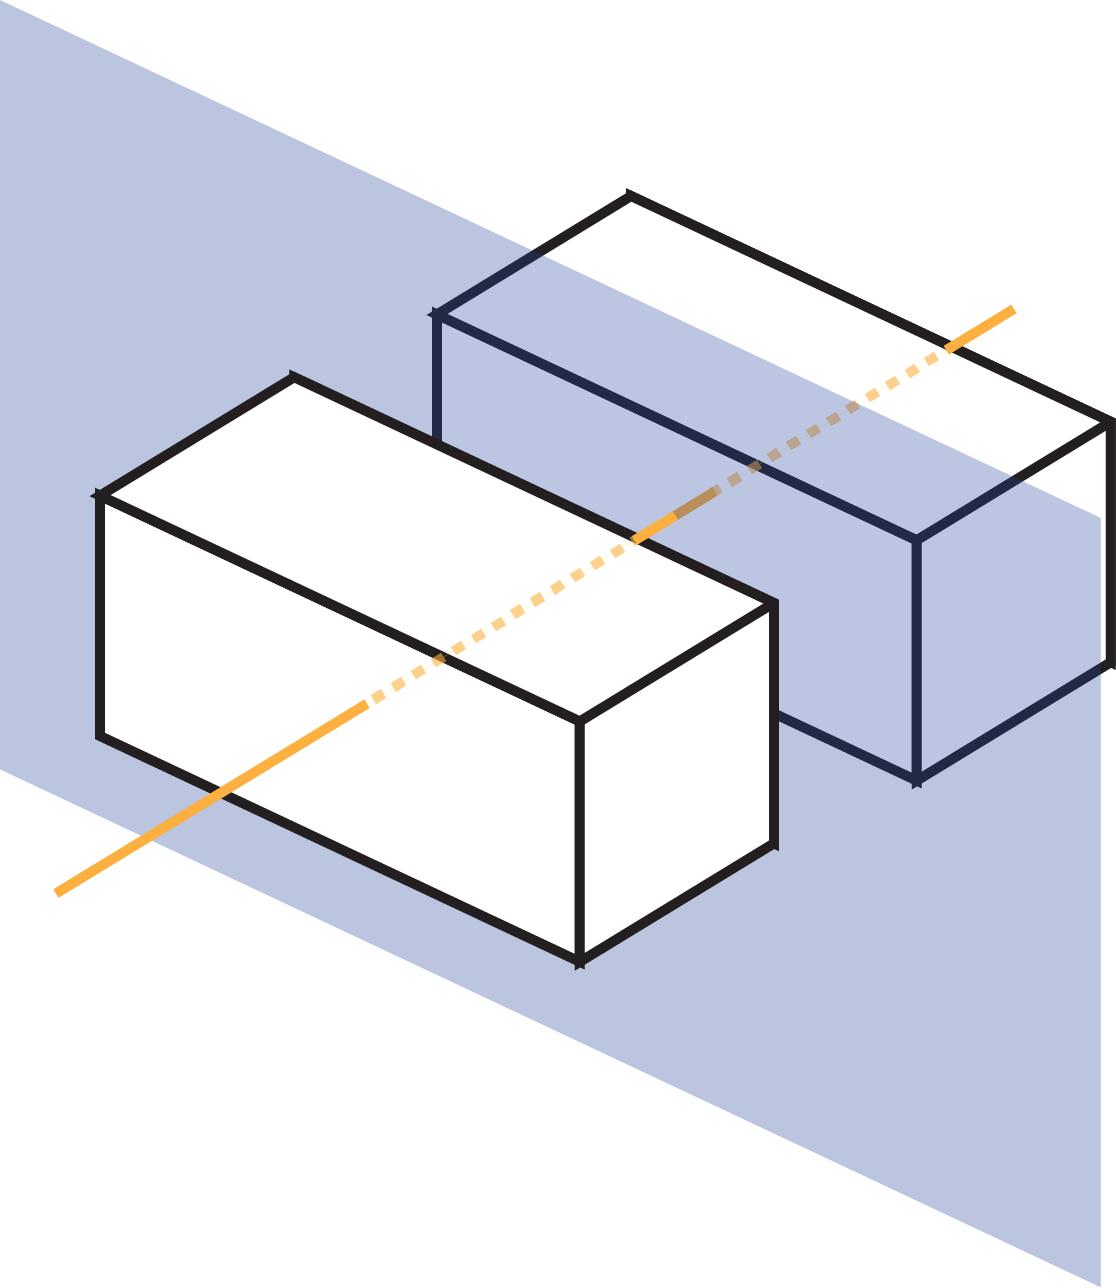
\includegraphics[width=\textwidth*\real{0.15}]{Images/z_axis_plane.png}
	}
	\qquad
	\subfloat[Parallel]{
        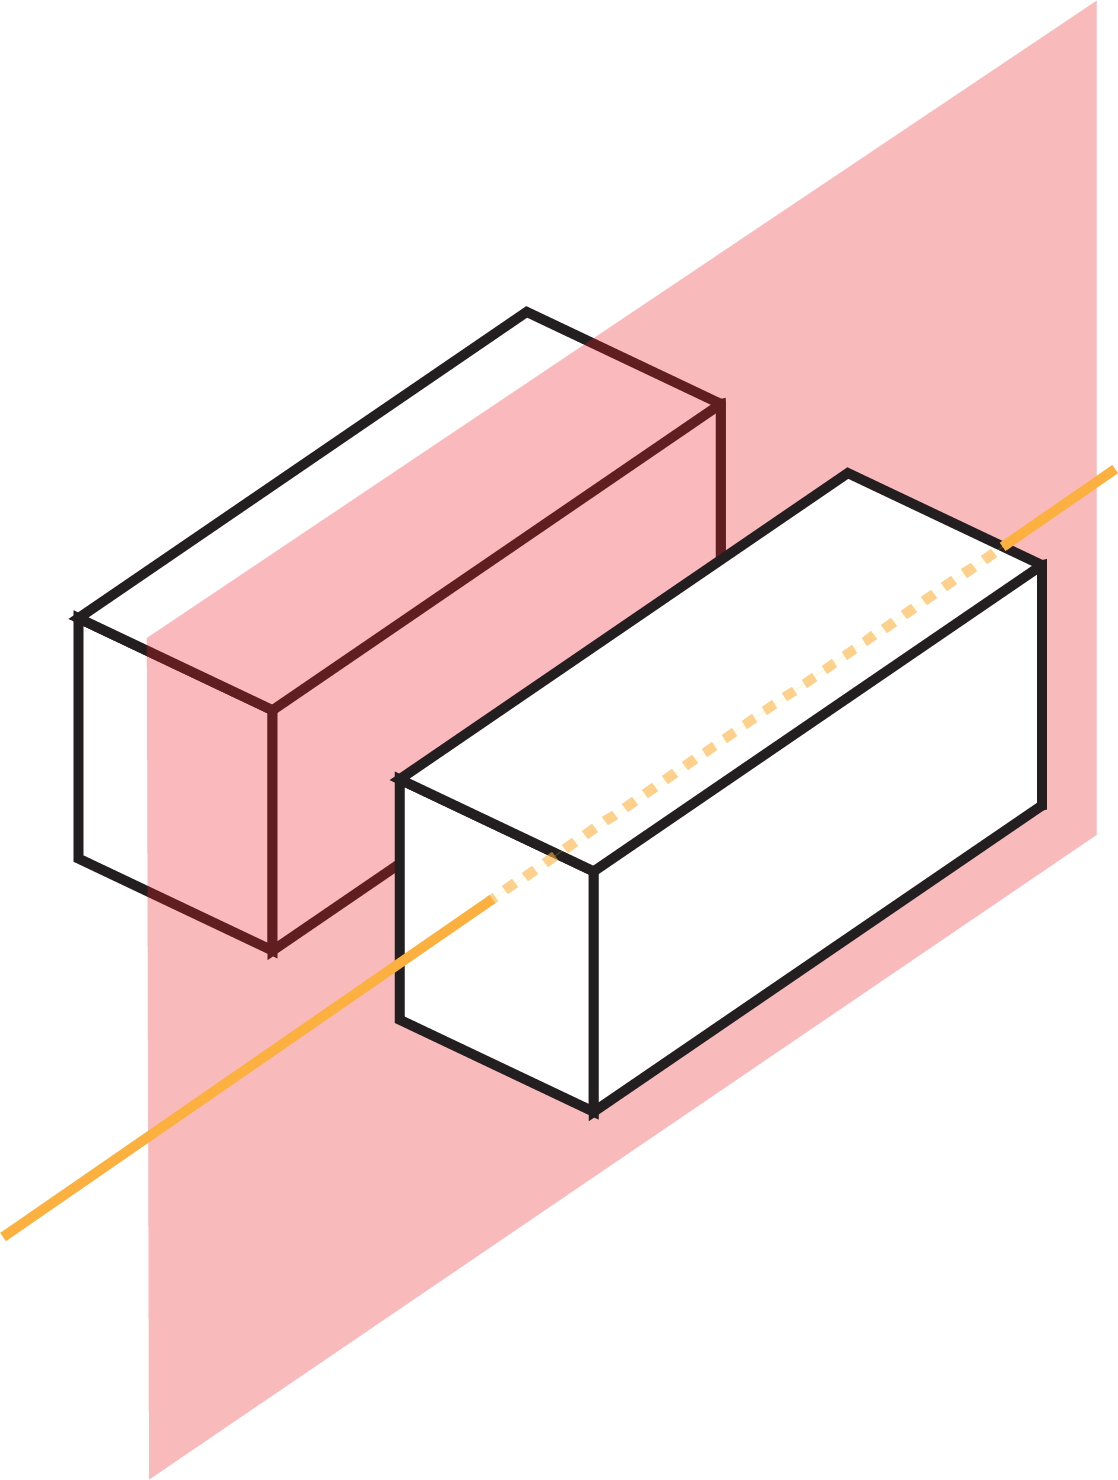
\includegraphics[width=\textwidth*\real{0.15}]{Images/x_axis_plane.png}
    }
    \caption{Splitting plane orientation.}
    \label{fig:splitting_overlap}
\end{figure}

In our implementation, better described in the relative section, for each one of the possible three splitting plane orientations, we assign a value telling the builder \textit{how much parallel} a plane is to the rays of the ray distribution the AABB is placed into. The builder will then try the splitting plane with the highest value, and use PAH to find the actual best cut.

\section{Top Level Structure}
In the previous sections, we summarized the two novel heuristics we propose. In this section, we will introduce two structures that can be used to enable the adoption of our heuristics in a concrete case.

In case we use SAH and LSPH, a single BVH can be built for the entirety of the scene, because the heuristics do not depend on local properties of the scene. However, PAH and SPFH do depend on artifacts in the ray distribution, which are localized in specific regions of the scene. In particular, in order to delimit the region where a parallel ray distribution is present, we use an Oriented Bounding Box; whereas, for a radial distribution we use a 3D frustum. 

\begin{figure}[H]
    \centering 
    \subfloat[OBB]{
        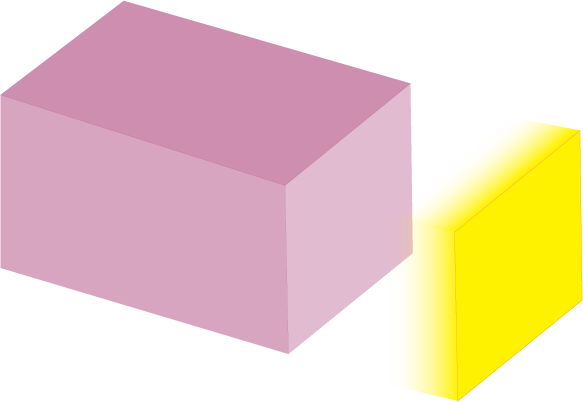
\includegraphics[width=\textwidth*\real{0.15}]{Images/obb_3d.png}
	}
	\qquad
	\subfloat[Frustum]{
        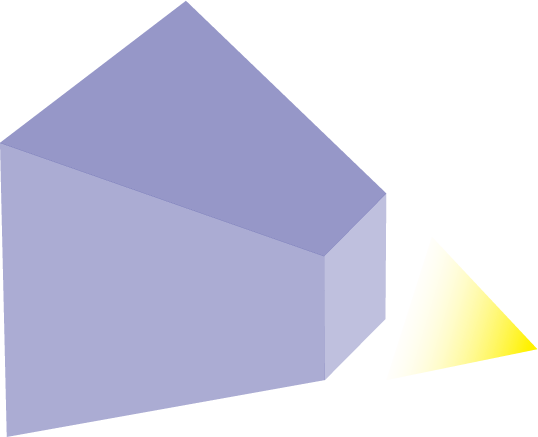
\includegraphics[width=\textwidth*\real{0.13}]{Images/frustum_3d.png}
    }
    \caption{Regions.}
    \label{fig:regions}
\end{figure}

In our thesis, we refer to the regions where a relevant ray distribution is present respectively with the terms \textit{plane influence area} and \textit{point influence area}.

Each influence area has an associated local BVH, built with PAH and SPFH, that can be traversed to find the rays-scene intersection for a ray \textit{affine} with the underlying ray distribution. With the term \textit{affine} we require two conditions:
\begin{itemize}
    \item The ray origin must be inside the influence area;
    \item The ray direction must be \textit{almost parallel} to the direction of the rays in the influence area.
\end{itemize}

The second condition is easy to verify for plane influence areas, where a dot product and a threshold can be used. For point influence areas, the test is a bit more complex, but an intuition of it can be seen in the image below:

\begin{figure}[H]
    \centering
    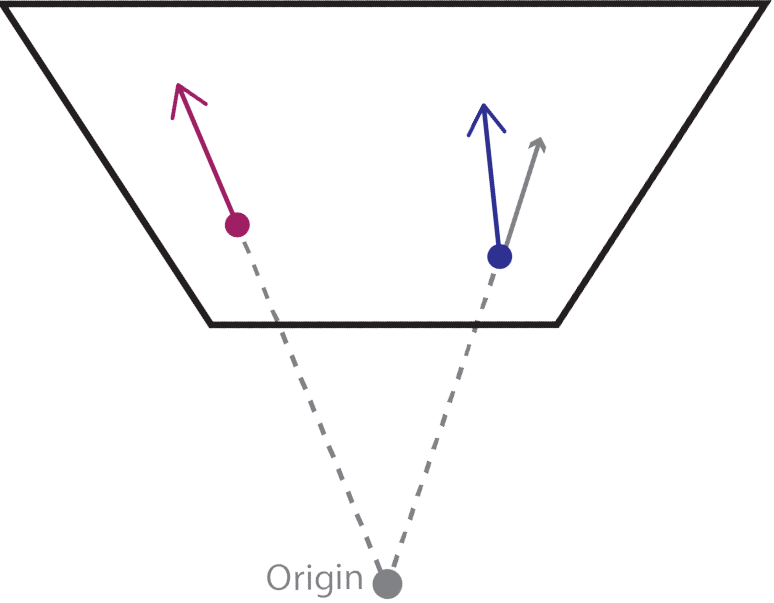
\includegraphics[width=\textwidth*\real{0.2}]{Images/direction_affinity.png}
    \caption{Blue ray is not affine, purple is.}
    \label{fig:direction_affinity}
\end{figure}

The first condition, instead, can be in principle verified with well-known point-OBB or point-frustum inside tests. However, as the number of influence areas increases, performing these tests doesn't scale. For this reason, we decided to implement an octree structure to make the time to find the appropriate influence areas constant. We approximate the influence areas with the nodes of the octree, and then traverse it to its leaves to find out what influence areas are present in a discrete region of the space.

Last, we must make sure that, even for rays that are not affine to any influence area, or rays that do not find an intersection in the local BVH, it is possible to find if and where they hit the scene. In order to do so, we can build a global BVH with state-of-the-art heuristics over the remaining geometry of the scene, which we call fallback BVH. If too many rays have to fall back to the global BVH, it means that using the local BVH is not necessary. In our work, we propose a formula to compute a threshold telling the maximum percentage of rays using the fallback BVH for our heuristics to be useful.

\begin{figure}[H]
    \centering
    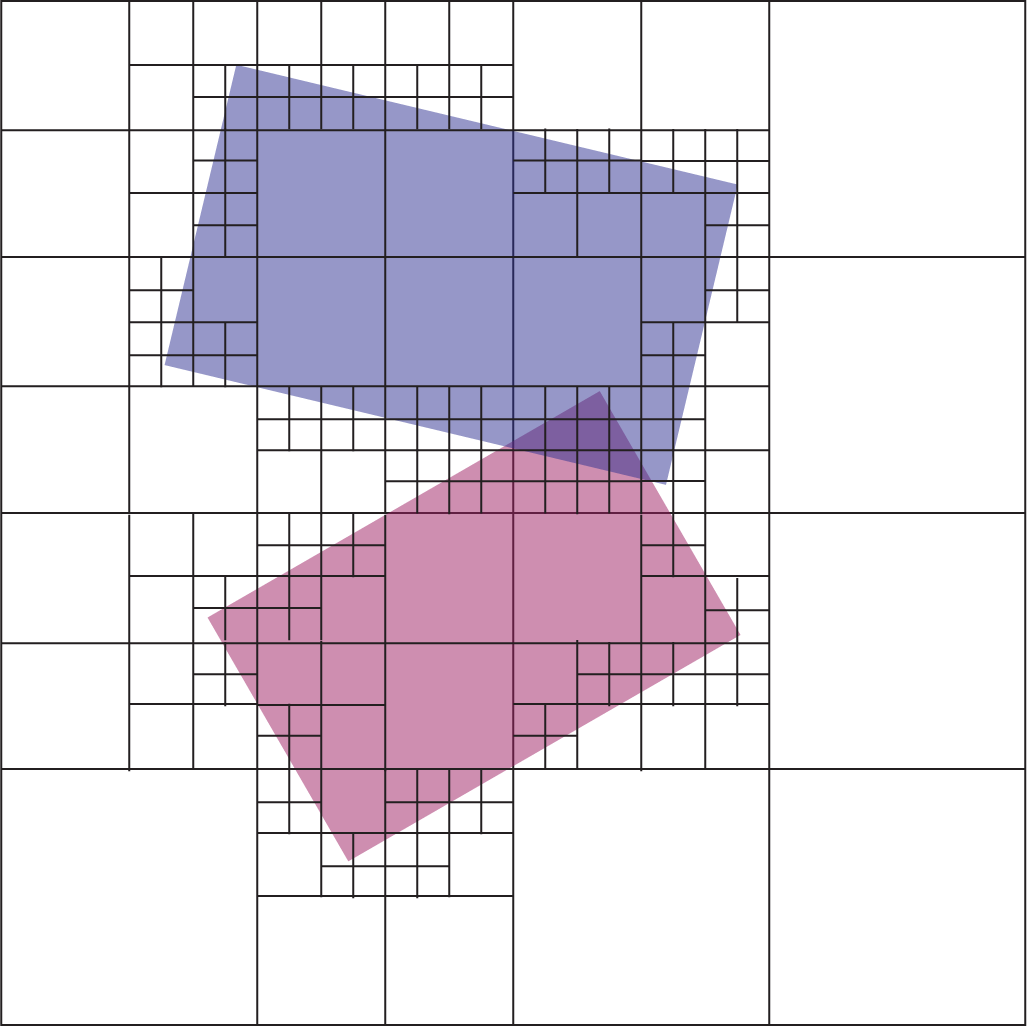
\includegraphics[width=\textwidth*\real{0.27}]{Images/octree_for_influence_areas.png}
    \caption{2D octree visualization.}
    \label{fig:octree_for_influence_areas}
\end{figure}

\section{Implementation}
In this section we will briefly talk about the implementation of the framework we used to carry out experiments to verify our heuristics. We have also implemented a visualizer in Unity, however it is outside the scope of the thesis.

We decided to implement the algorithms in C++23, and we followed two guiding principles:
\begin{itemize}
    \item Build a framework that can be easily used by other users to test different case scenarios, or even modify the implementation;
    \item Have full control over the code, in order to be able to understand better the results.
\end{itemize}

In order to follow the first principle, we designed our algorithms in a modular way, so that it is easy to change only some parts of the code (for example by using lambdas), or to extract different aspects of the results, for an easier analysis.

For what concerns the second principle, we decided to implement all the code on our own, following the state-of-the-art core concepts, but without optimizing them or using external libraries.

\subsection{BVH}
In our algorithm, the BVH construction is split into these phases:
\begin{description}
    \item[Splitting plane orientation choice] The orientation of the splitting plane must be decided by using a heuristic (either our SPFH or standard LSPH);
    \item[Splitting plane position choice] Once the orientation is fixed, the algorithm starts trying different splitting plane positions. For each one, the cost of the two children is computed (by using our PAH or standard SAH). The best one is kept.
    \item[Cut evaluation] Based on some customizable thresholds, it is possible to decide whether the two children are good enough, or if it is worth it to try the second-best splitting plane orientation, or even fallback to using standard heuristics. 
    \item[Termination criterion] When to stop further subdividing nodes.
\end{description}

The strategies to decide the splitting plane orientation, cost function and termination criterion can be completely customized by injecting the functions the user wants to use, even self-made. The cut evaluation stage is instead fixed, but the various properties of the BVH can severely influence the decisions. Thanks to this design, not only it is possible to try different builders with predefined heuristics (for example oriented to quality or speed), but it is also possible to use user-defined heuristics and strategies.

\subsection{BVH Analyzer}
We implemented a class where it is possible to specify how to analyze the BVH. We decided to completely isolate the analysis from the construction, in order not to get results influenced by the properties we measure. In the \texttt{BvhAnalyzer} class, it is possible to specify a list of pairs of functions. The first element of the pair is executed for each node, but it is able to store data \textit{globally}. The second function is executed at the end of the BVH construction, and has access to the global data of the associated per-node function. For example, the per-node function can compute the amount of triangles each node has, increase a total counter and write it to a Json; the final function can print the total number of triangles. We used template metaprogramming to achieve this.

Since generated files can be huge, we also implemented a way to extract only specific data to a csv file.

\subsection{Top Level Structure}
The top level structure we implemented, apart from the naive one, is the octree. The octree is built on the influence areas, which are described by OBBs and frustums. The idea is that the node of the octree is a leaf only if the influence areas inside it are the same for all its extension, as can be observed in the image below:

\begin{figure}[H]
    \centering 
    \subfloat[Leaves]{
        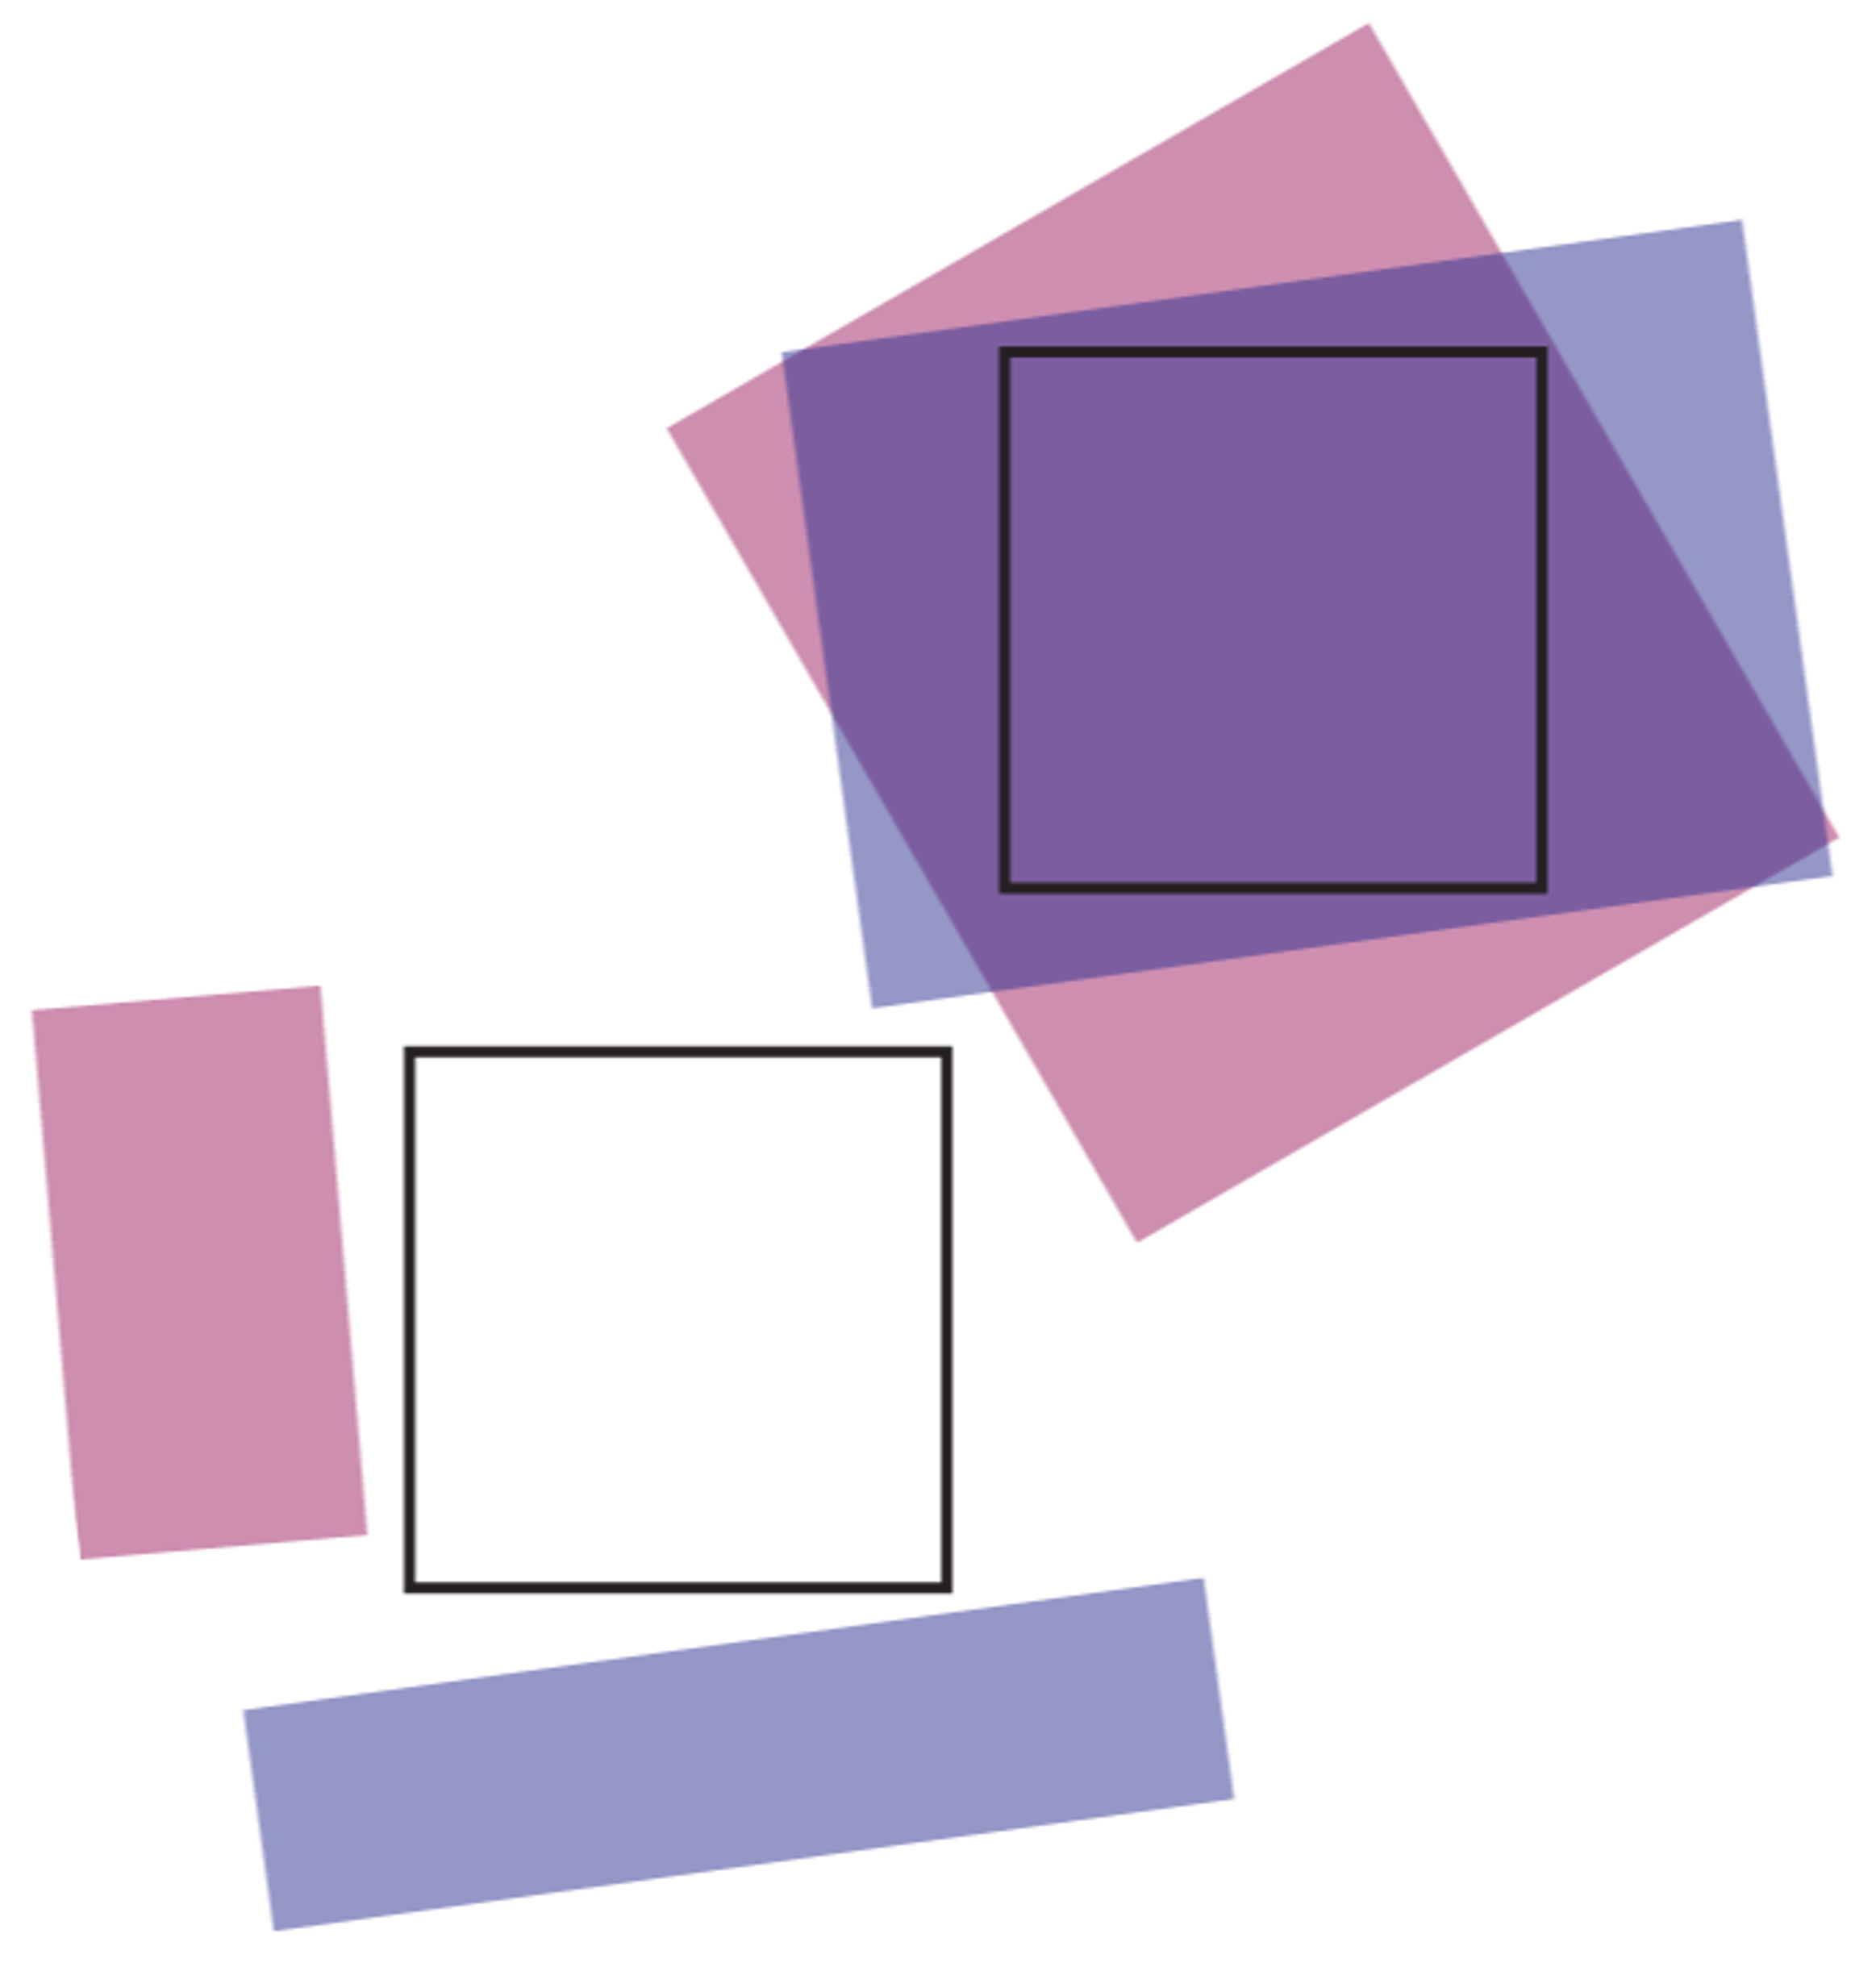
\includegraphics[width=\textwidth*\real{0.15}]{Images/leaf.png}
	}
	\qquad
	\subfloat[Not leaves]{
        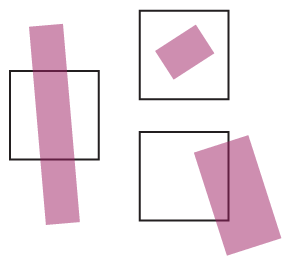
\includegraphics[width=\textwidth*\real{0.15}]{Images/non_leaf.png}
    }
    \caption{Octree leaf criteria.}
    \label{fig:leaves}
\end{figure}

The leaves only store the influence areas they contain. The octree is then traversed based on the ray origin, and the influence areas and their associated local BVHs can be retrieved and traversed. If a leaf contains multiple BVHs, it is possible to specify how many to traverse, in case no intersection is found in previous traversals. In our tests, we always use only the first BVH present in the leaf and, in case no intersections are found, we immediately fall back to the global BVH.

Also for the octree we developed an analyzer, although less sophisticated than the BVH one.

\section{Experimental Results}
We carried out tests to measure the quality and build time of the BVHs built with our heuristics, compared to the state-of-the-art ones. We also performed tests to compare some metrics among BVHs built with PAH and SPFH, but having different properties. Last, we measured how many levels of the octree are needed to have a good enough approximation of the influence areas, as well as how they compare to the naive method. We also performed a static analysis on the memory footprint of BVHs and octrees. Due to space constraints, we will only briefly mention the most important results in this document.

\subsection{BVH analysis}
The analysis of the BVHs has been carried out on 8 different scenes, each one with peculiar characteristics. In each test case, we created a single influence area, covering the majority of the scene. For each scene we executed 8 test cases: 4 with plane influence areas and 4 with point ones. For each influence area, we changed its orientation: parallel to one cartesian direction, 15°, 45° and oblique.

We started by performing tests where both PAH and SPFH are used. We first measured the accuracy of PAH in estimating the cost of the BVH. To do so, we developed a way to measure the actual cost of the traversal of a BVH, and compared it to the cost estimated by PAH. To measure the real cost of a BVH, we traverse it with rays and, for each ray intersection with an AABB, we compute its cost as $\#triangles \cdot K$. This cost function is the same as the PAH cost function, without the probability part, which is intrinsically taken into account by the fact that we are actually tracing rays. We found out that PAH is extremely accurate at estimating a BVH cost: its average error is $7\%$, whereas SAH's is $36\%$.

We then used the real cost of the traversal, computed as explained above, and compared it to the cost of BVHs built with SAH and LSPH over the exact same geometry. The results showed that our heuristics combined, cannot produce better BVHs than state-of-the-art, except when rays are parallel to one cartesian axis.

We therefore decided to test both heuristics in isolation: the take-away point is that SPFH produces higher-quality BVHs than state-of-the-art, especially in the test cases where rays are parallel or \textit{almost parallel} to a cartesian axis, as it can be observed in chart \ref{fig:spfh_iso_chart}. 

\begin{figure}[H]
    \centering
    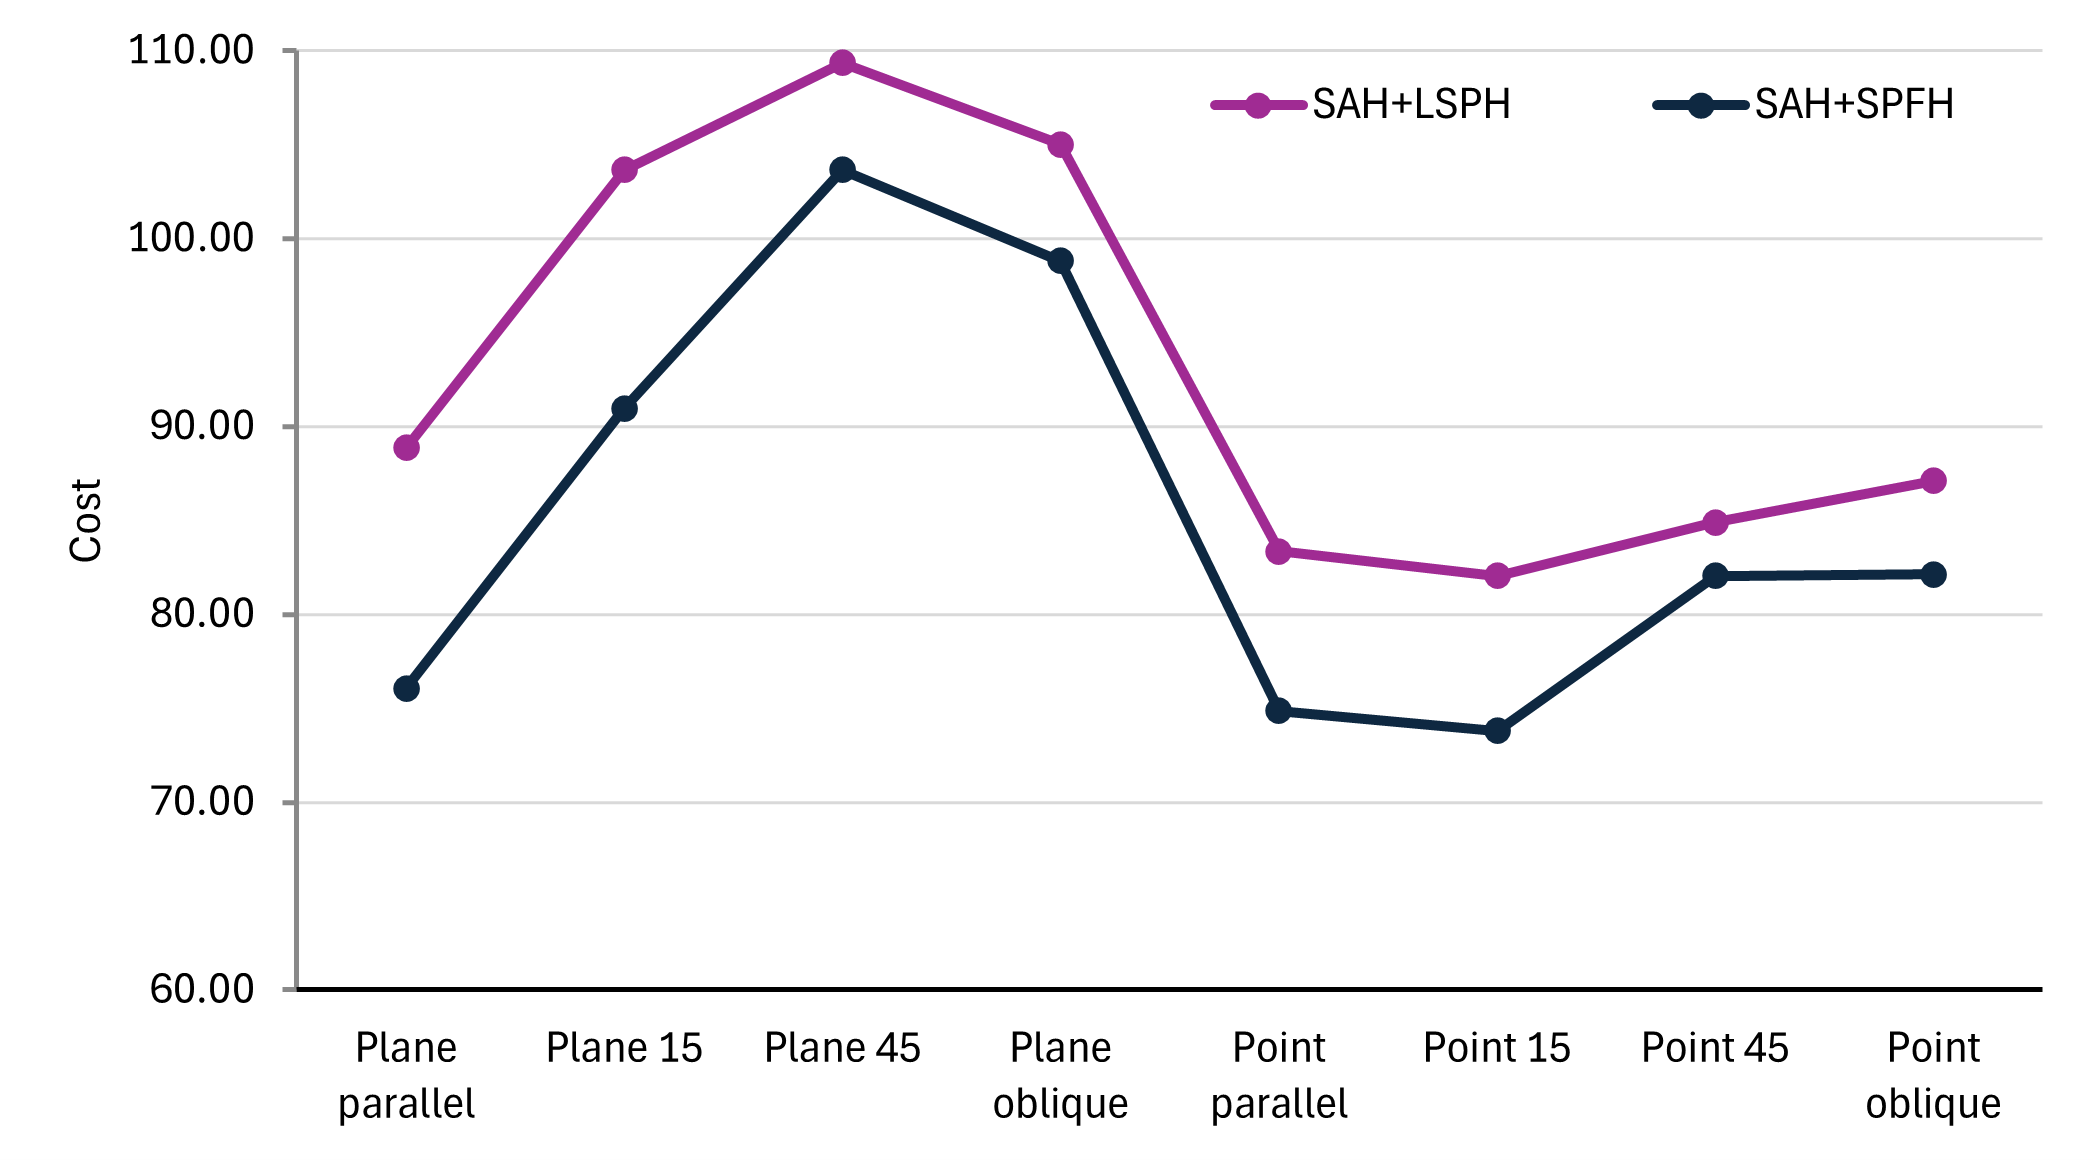
\includegraphics[width=\textwidth*\real{0.47}]{Images/spfh_isolation.png}
    \caption{SPFH vs LSPH.}
    \label{fig:spfh_iso_chart}
\end{figure}

On the other hand, PAH cannot match state-of-the-art performance, despite it being a way more accurate measurement of BVH quality. The main drawback of PAH is that, when the projections of the sibling nodes overlap, it tends to produce very unbalanced BVHs.

We also measured the time required to use PAH and LSPH. We found out that PAH is an order of magnitude slower than SAH. On the other hand, SPFH is on average as fast as LSPH.

Eventually, we decided to analyze BVHs built with our heuristics, but different properties. The properties mainly interact with how picky the algorithm is with the choosing of the splitting plane. By analyzing different options, we empirically detected the best values to have a good balance between build speed and quality. 

Unluckily this analysis and the one on the memory footprint cannot be presented here.

\subsection{Top Level Structure}
While measuring the performance of the octree, we were interested in comparing them with the naive method in a scenario where there are a lot of influence areas, and in a scenario with few influence areas. As we expected, as the number of influence areas increases, the naive method scales badly, whereas the octree remains constant. Already with 8 influence areas, an octree with 5 levels is faster than the naive method.

We then carried out analyses to find out the optimal number of levels for the octree:

\begin{figure}[H]
    \centering
    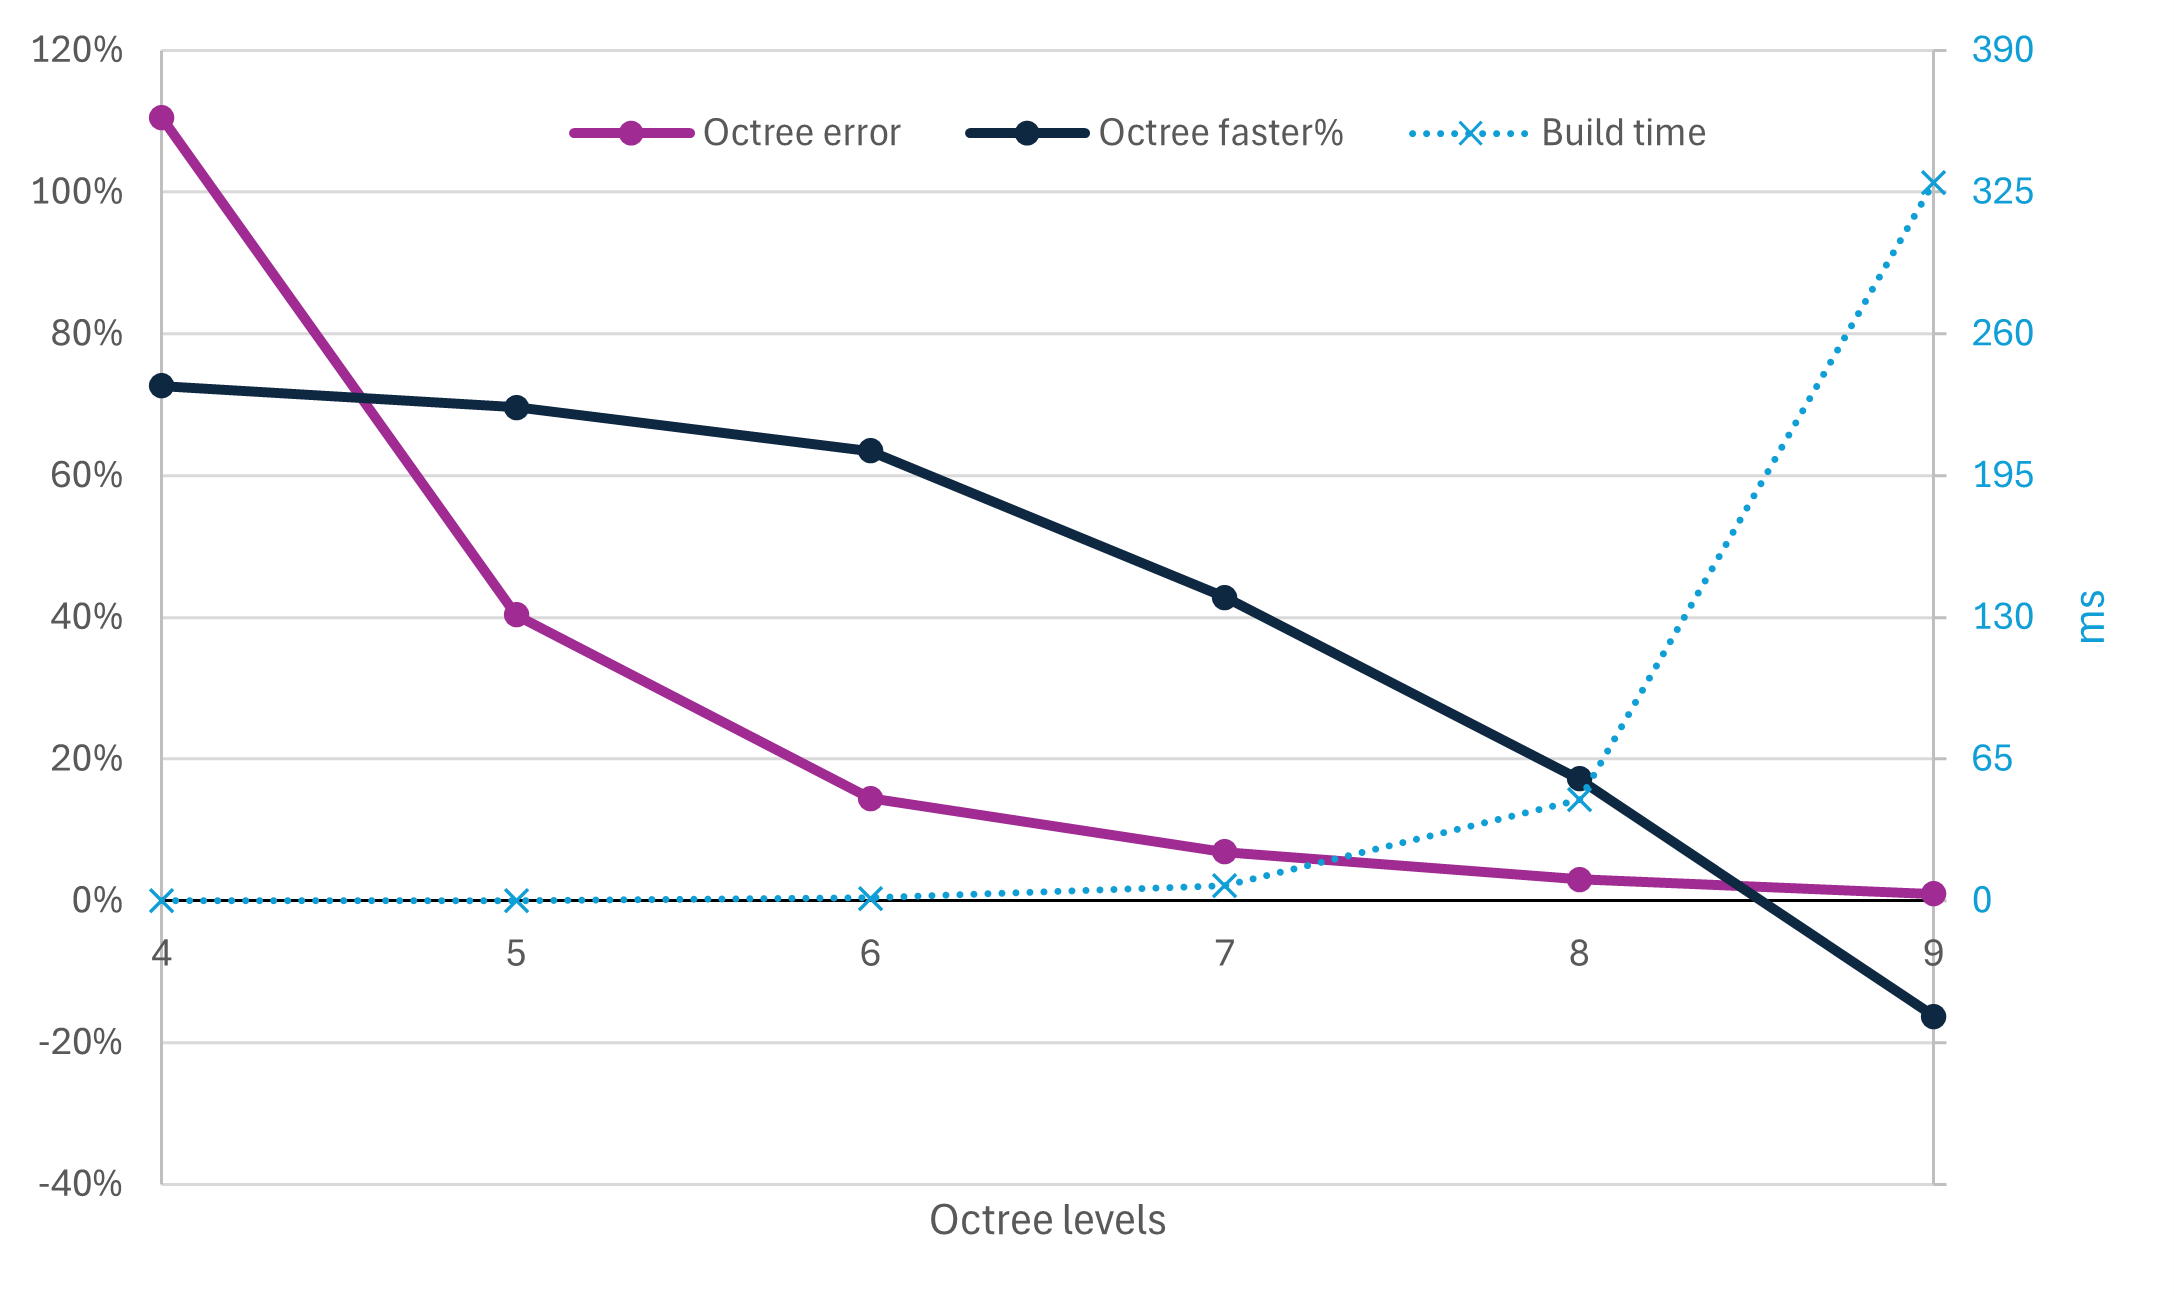
\includegraphics[width=\textwidth*\real{0.47}]{Images/octree_error_faster_chart.png}
    \caption{Octree error vs speed.}
    \label{fig:octree_levels}
\end{figure}

As it is possible to observe, as the number of levels increases, the error decreases. With the term error, we refer to the fact that an octree approximates the influence areas with cubic blocks. The octree approximation is conservative, which means that it can consider a point inside a region even if it is not, but never the opposite. Of course, an octree with more levels is exponentially slower to traverse and build. By looking at the graph we decided to use 5-level octrees in our tests, even though the maximum difference between error and speed would be with 6-level octrees.

\section{Conclusions}
Many future development directions can be studied. The most important direction would be to try to tweak PAH in order to avoid its main drawback, which we described above. Future researchers may also try to improve the algorithms of our framework, in order to optimize them and, ultimately, run them on a parallel architecture like a GPU. Another important development would be to write a clustering algorithm to automatically identify the relevant ray distributions in the 6-dimensional space of the scene.

\rule{0.471\textwidth}{0.5pt}

In our thesis, we propose two novel heuristics to build higher-quality BVHs, by leveraging some artifacts in the ray distribution produced by Monte-Carlo importance sampling. The experimental results, obtained by running our implementation on many different test cases, show how, when the influence areas have rays parallel to a cartesian axis, SPFH produces a BVH with a lower traversal cost than state-of-the-art heuristics, without it being more expensive. Whereas PAH, in isolation, is not better than SAH, but can be used to better estimate the cost of a BVH without tracing any ray, thanks to its high accuracy.

\end{document}